\chapter{Metodologia}\label{ch:metodologia}

% ============================================================
%  VISÃO GERAL DO CAPÍTULO
% ============================================================

% \section{Projeto geral}\label{sec:diseno_general}

A metodologia consiste em caracterizar a distribuição espacial e a magnitude dos máximos de precipitação e vento associados aos ciclones extratropicais do Atlântico Sul, adotando um referencial lagrangiano centrado no sistema.
A análise é condicionada sistematicamente por dois fatores: a fase do ciclo de vida e a região de ciclogênese.
A estratégia segue a sequência lógica de cinco etapas: (1) definição das fontes de dados; (2) construção e estratificação das populações de ciclones; (3) processamento lagrangiano dos campos de superfície; (4) caracterização estatística univariada por meio de estimação de densidade e análise EOF; e (5) análise multivariada (MEOF) e construção de protótipos estruturais.
Os protótipos são organizados em painéis $3 \times 4$ (3 regiões de ciclogênese $\times$ 4 fases evolutivas) para a População Global e o subconjunto p90.

% ============================================================
%  SEÇÃO M1 — DADOS
% ============================================================

\section{Dados}\label{sec:datos}

\subsection{Reanálise ERA5}\label{sec:datos_era5}

Para a caracterização dos campos de superfície, utilizou-se a reanálise de quinta geração do ECMWF, ERA5 \citep{hersbach2020era5}, acessando especificamente o conjunto de dados \textit{``ERA5 hourly data on single levels from 1940 to present''} \citep{hersbach_era5_2023b} para o período 1979--2020.
A justificativa da escolha do ERA5, incluindo sua resolução espacial ($\sim$31 km) e temporal (horária) e sua representação superior da intensidade ciclônica no Atlântico Sul em relação a gerações anteriores de reanálises \citep{gramcianinov2020analysis}, foi apresentada na Introdução e nos Fundamentos (Seção~\ref{sec:tb_fundamentos}).
No entanto, deve-se reconhecer uma limitação documentada na representação de extremos: \citet{chen2024evaluation} demonstram que o ERA5 subestima sistematicamente os extremos dos 5\% de ciclones extratropicais mais intensos, com vieses de $-10{,}2\%$ no vento e $-22{,}6\%$ na precipitação em relação às observações nos Estados Unidos da América.
Isso implica que os resultados obtidos para p90 devem ser interpretados como estimativas conservadoras da intensidade real dos eventos.

\subsection{Variáveis meteorológicas}\label{subsec:variables}

A análise foi realizada a partir de campos horários extraídos do ERA5, utilizando as seguintes variáveis de superfície:

\begin{itemize}
    \item Precipitação total acumulada (\texttt{tp}, em mm\,h$^{-1}$).
    \item Magnitude do vento em superfície a 10 m (\texttt{wind10}, em m\,s$^{-1}$).
\end{itemize}

A caracterização de ambas as variáveis responde à natureza morfológica dos ciclones extratropicais e sua respectiva estrutura dos campos de precipitação e vento, fundamentada na Seção~\ref{subsec:tb_compound_def} dos Fundamentos.
Este enfoque permite descrever a configuração espacial típica dos campos de superfície em cada fase evolutiva, permitindo avaliar a eventual coocorrência dos máximos de ambas as variáveis.
Esta estratégia é a primeira abordagem à análise multivariada (MEOF) posterior, detalhada na Seção~\ref{subsec:eof_multivariado}.

\subsection{Base de trajetórias e fases}\label{sec:bd_ciclones}
O ponto de partida para a caracterização dos sistemas é o catálogo de trajetórias desenvolvido por \citet{gramcianinov2019properties} a partir da reanálise ERA5, cuja alta resolução permite capturar sistemas de mesoescala e ciclogênese na região de estudo.
Os parâmetros de configuração do algoritmo de rastreamento e os filtros aplicados são detalhados na Tabela~\ref{tab:tracking_params}.

\begin{table}[ht]
\centering
\caption[Parámetros y filtros de la base de trayectorias]{Parámetros técnicos y filtros aplicados en la base de datos de trayectorias \citep{gramcianinov2020analysis}.}
\label{tab:tracking_params}
\begin{tabular*}{\textwidth}{@{\extracolsep{\fill}}ll}
\hline
Parámetro & Especificación \\ 
\hline
Fuente de datos & ERA5 (ECMWF) \\
Resolución espacial & $\sim$31 km ($0.25^\circ \times 0.25^\circ$) \\
Variable de seguimiento & Vorticidad relativa en 850 hPa ($\zeta_{850}$) \\
% % Nivel de filtrado espectral & T42 (para aislar la escala sinóptica) \\
% % Umbral de intensidad & $\zeta_{850} < -1.0 \times 10^{-5}$ s$^{-1}$ \\
Duración mínima & 24 horas \\
Desplazamiento mínimo & 1000 km \\ 
\hline
\end{tabular*}
\end{table}

% \begin{table}[ht]
% \centering
% \caption{Parámetros técnicos y filtros aplicados en la base de datos de trayectorias \citep{gramcianinov2019properties}.}
% \label{tab:tracking_params}
% \begin{tabular*}{\textwidth}{@{\extracolsep{\fill}}ll}
% \hline
% Parámetro & Especificación \\ 
% \hline
% Fuente de datos & ERA5 (ECMWF) \\
% Resolución espacial & $\sim$31 km ($0.25^\circ \times 0.25^\circ$) \\
% Variable de seguimiento & Vorticidad relativa en 850 hPa ($\zeta_{850}$) \\
% % % Nivel de filtrado espectral & T42 (para aislar la escala sinóptica) \\
% % % Umbral de intensidad & $\zeta_{850} < -1.0 \times 10^{-5}$ s$^{-1}$ \\
% Duración mínima & 24 horas \\
% Desplazamiento mínimo & 1000 km \\ 
% \hline
% \end{tabular*}
% \end{table}


Sobre esta base, \citet{coutodesouza2024new} processaram o catálogo incorporando uma classificação objetiva das fases evolutivas por meio do algoritmo \textit{CycloPhaser} \citep{deSouza2025CycloPhaser}, o qual avalia a taxa de variação da vorticidade relativa em 850 hPa ($\zeta_{850}$) para segmentar matematicamente os momentos de desenvolvimento e decaimento de cada sistema.
Os fundamentos físicos que justificam tanto a escolha de $\zeta_{850}$ como variável de \textit{tracking} quanto a segmentação do ciclo de vida em quatro fases são expostos nas Seções~\ref{subsec:tb_zeta} e~\ref{subsec:tb_fases} dos Fundamentos. A Tabela~\ref{tab:fases_def} resume tais fases.

\input{tabelas_es/tab_fases_def.tex}

% ============================================================
%  SEÇÃO M2 — POPULAÇÕES DE ESTUDO
% ============================================================

\section{Construção das populações de estudo}\label{sec:poblaciones_estudio}

A segmentação da amostra segue os critérios explicados na Seção~\ref{subsec:tb_poblaciones} dos Fundamentos.
A base de dados de trajetórias foi dividida em duas: uma população de referência (População Global) e, a partir dela, um subconjunto de alta intensidade ($p90$).
Ambas as populações foram construídas de forma independente para cada uma das três regiões de ciclogênese (SBR, LPB e ARG), cuja delimitação espacial segue a taxonomia proposta por \citet{gramcianinov2019properties} e é detalhada na Tabela~\ref{tab:regiones_coords}.
A estratificação geográfica responde ao fato de que essas regiões apresentam regimes dinâmicos diferenciados, cujas características físicas foram discutidas na Seção~\ref{sec:tb_regiones} dos Fundamentos.

\input{tabelas_es/tab_regiones_coords.tex}

\subsection{População Global: climatologia de referência}\label{subsec:grupo_global}

A População Global estabelece o comportamento morfológico e estatístico médio dos ciclones com um desenvolvimento típico e completo na região.
Para compô-la, aplicou-se um critério de coerência evolutiva à base de ciclones, selecionando unicamente os sistemas que cumpriram dois critérios simultâneos:

\begin{enumerate}
    \item Ciclo de vida completo: Presença confirmada e sequencial das quatro fases de desenvolvimento ---incipiente (\textit{incipient}), intensificação (\textit{intensification}), maturidade (\textit{mature}) e decaimento (\textit{decay})---.
    \item Ausência de fases complexas: Exclusão categórica de sistemas que desenvolveram fases secundárias, de reintensificação (e.g., \textit{intensification~2}, \textit{mature~2}) ou fases residuais (\textit{residual}).
\end{enumerate}

Isso elimina o ruído introduzido por sistemas efêmeros ou de evolução errática.
Para cada ciclone da População Global, identificou-se o registro temporal correspondente à sua máxima intensidade ---o extremo absoluto de vorticidade relativa a 850 hPa, $\zeta_{850}^{\min}$--- como métrica de intensidade para a segmentação posterior.

A Figura~\ref{fig:loc_vort_global} sintetiza a densidade de probabilidade da localização onde os ciclones da População Global alcançam seu $\zeta_{850}^{\min}$ ao longo de seu ciclo de vida, utilizando o número de ciclones detalhado na Tabela~\ref{tab:conteo_ciclones}.

\begin{figure}[htbp]
\centering
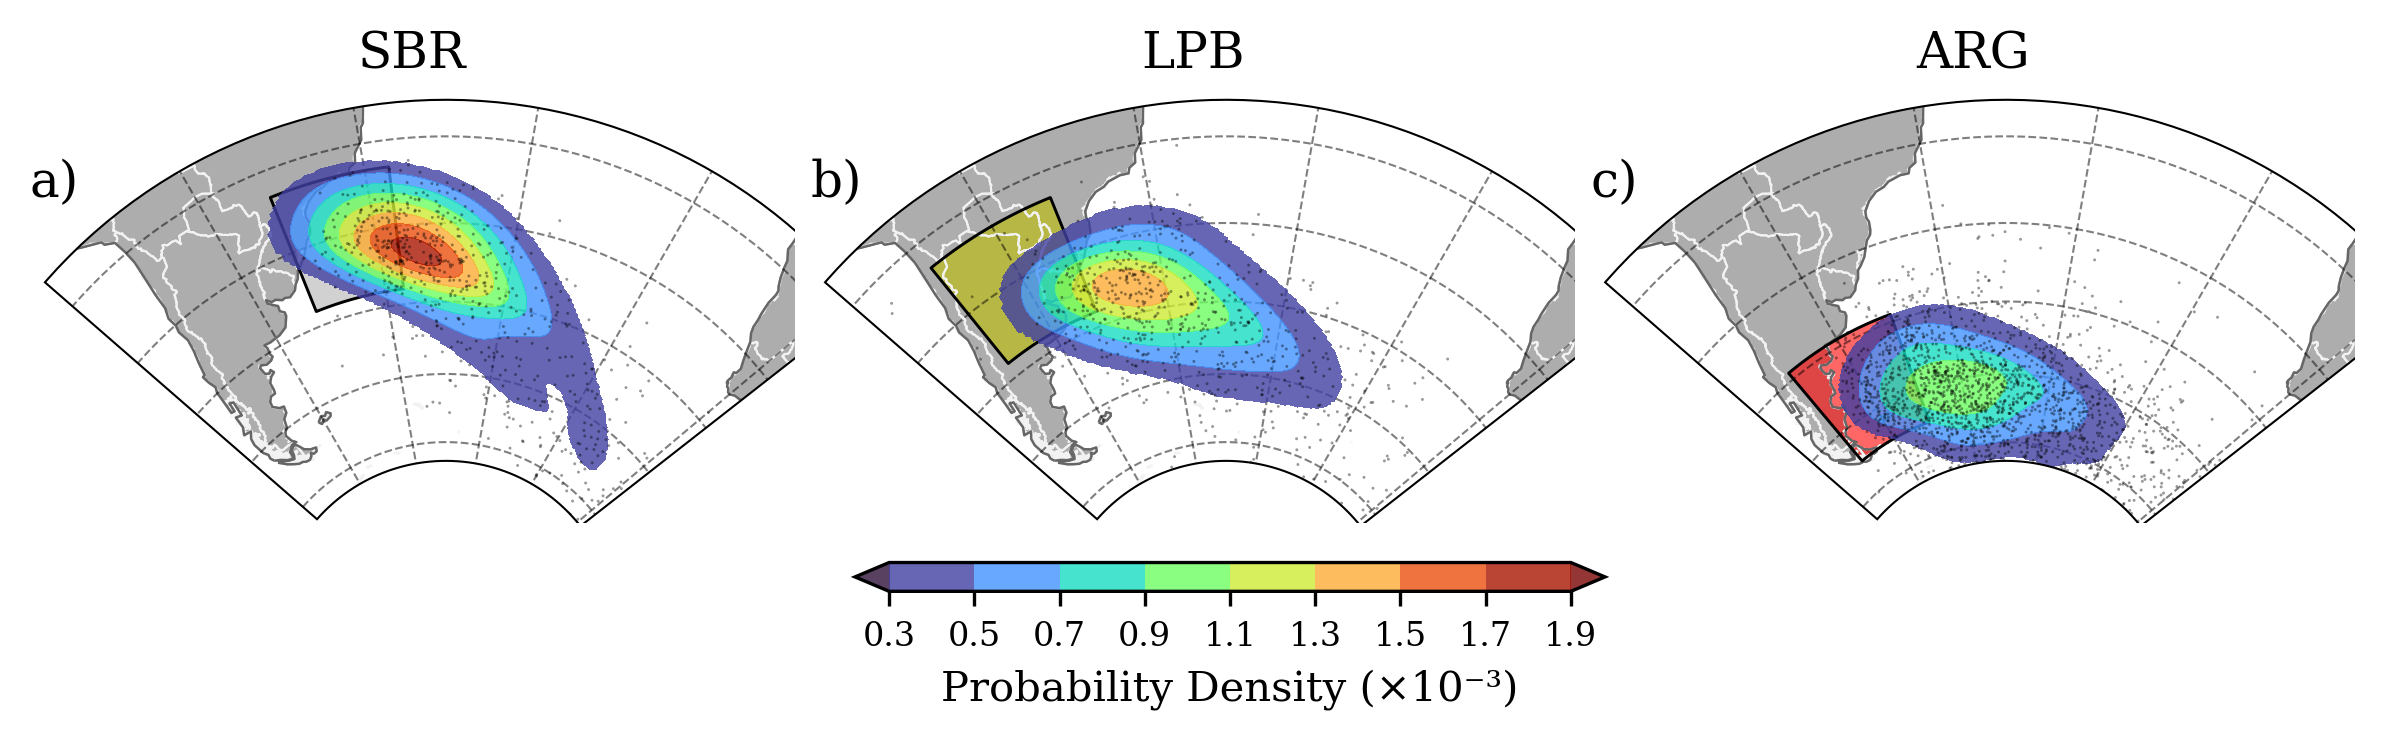
\includegraphics[width=\textwidth]{images/geral/vort_global_vf.png}
\caption[Localização do mínimo de vorticidade (População Global)]{Distribuição espacial da densidade de probabilidade da localização onde os ciclones da População Global alcançam sua menor vorticidade relativa a 850~hPa ($\zeta_{850}^{\min}$) ao longo de seu ciclo de vida. a), b) e c) correspondem às regiões de ciclogênese SBR, LPB e ARG, respectivamente. Os contornos coloridos indicam a densidade de probabilidade ($\times 10^{-3}$) e os pontos cinzentos marcam as posições individuais dos mínimos.}
\label{fig:loc_vort_global}
\end{figure}


\subsection{Subconjunto de alta intensidade (p90)}\label{subsec:subconjuntos_intensidad}

Para avaliar os padrões espaciais frente à severidade dinâmica do sistema, extraiu-se da População Global os 10\% de ciclones com os valores mais negativos de $\zeta_{850}^{\min}$, correspondentes a um decil da distribuição, obtendo o subconjunto $p90$ (explicado com mais detalhe em \ref{subsec:tb_poblaciones}).

A Tabela~\ref{tab:conteo_ciclones} documenta a redução do tamanho amostral desde a base bruta até a conformação da População Global e do subconjunto p90.

\input{tabelas_es/tab_conteo_ciclones.tex}

A análise da fase em que se registra o pico de vorticidade (Tabela~\ref{tab:fase_max_intensidad}) confirma que o subconjunto p90 respeita a estrutura dinâmica dominante: aproximadamente 83\% dos casos alcançam seu mínimo de intensidade durante a fase de maturidade, frente a menos de 5\% durante a fase de decaimento.

\input{tabelas_es/tab_fase_max_intensidad.tex}

Para completar a caracterização do subconjunto p90, a Figura~\ref{fig:loc_vort_p90} mostra a distribuição espacial da densidade de probabilidade da localização de seu mínimo de vorticidade.

% Figura para o subconjunto p90 (Subseção 2)
\begin{figure}[htbp]
\centering
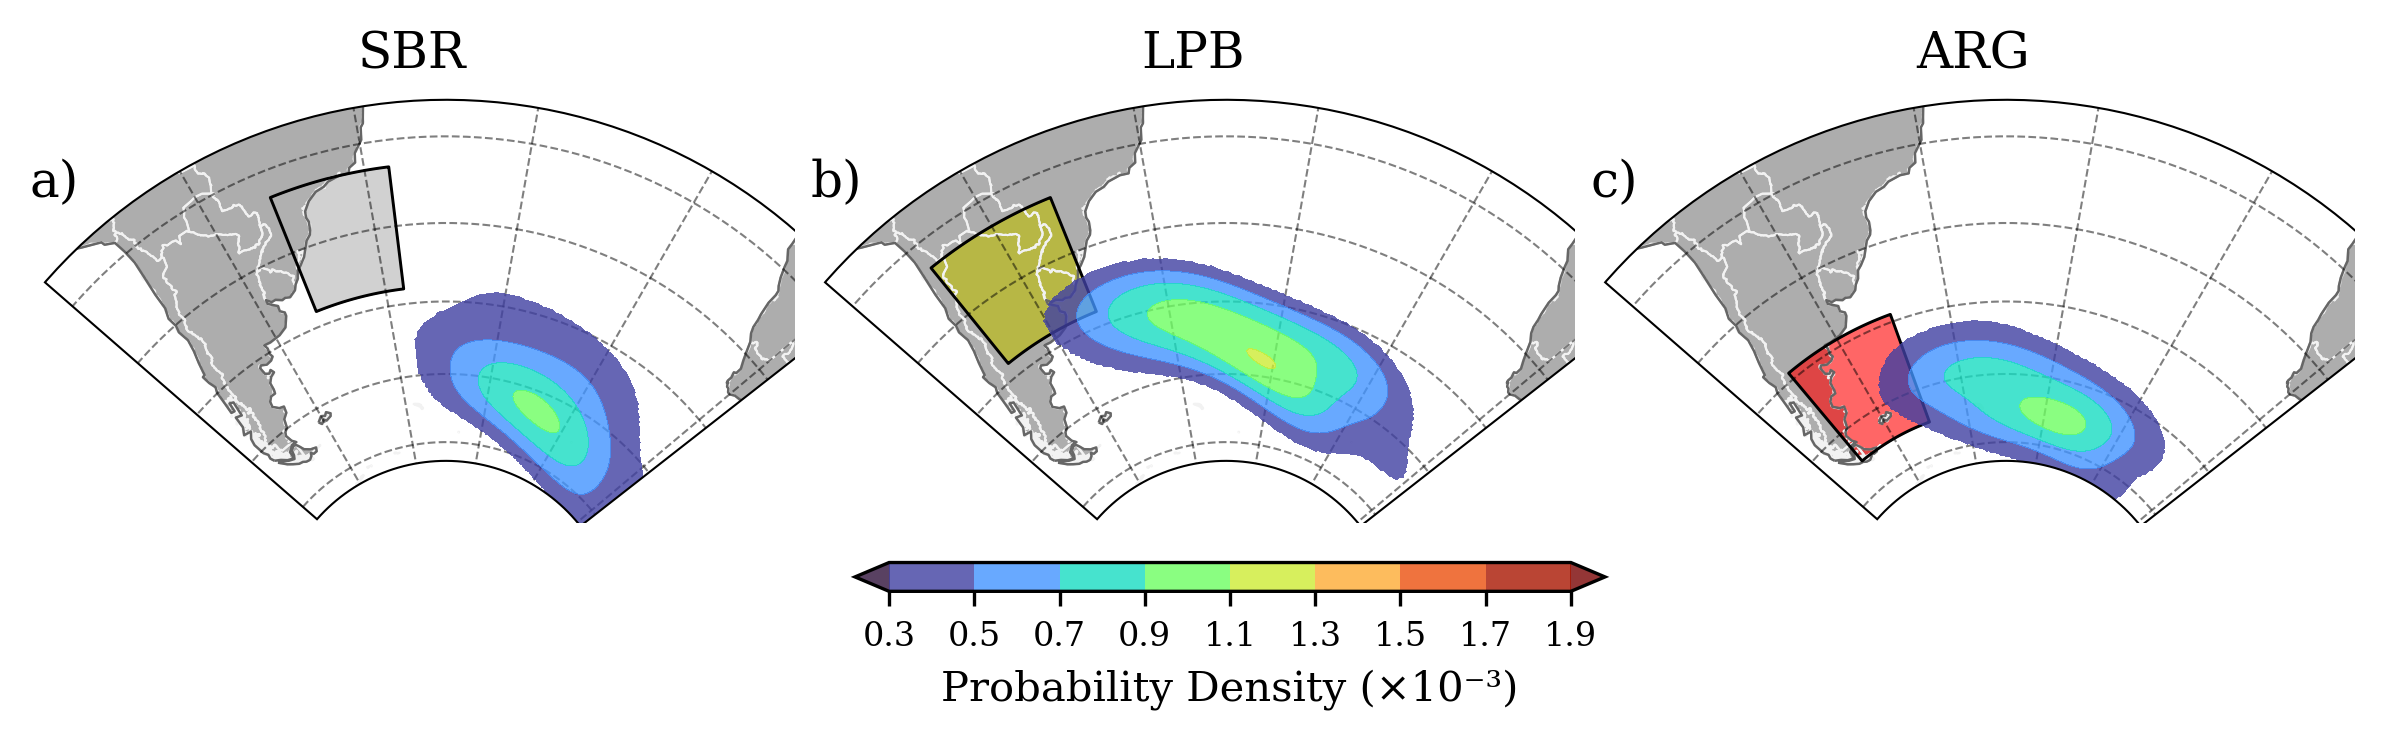
\includegraphics[width=\textwidth]{images/geral/vort_p90_vf.png}
\caption[Localização do mínimo de vorticidade (subconjunto p90)]{Similar à Figura~\ref{fig:loc_vort_global}, mas para o subconjunto p90 (sistemas mais intensos, decil inferior de $\zeta_{850}^{\min}$).}
\label{fig:loc_vort_p90}
\end{figure}

% \subsection{Análise comparativa}\label{subsec:estrategia_analise}

Sobre o subconjunto p90 ---e comparando-o sistematicamente com a População Global--- aplica-se integralmente o fluxo metodológico descrito nas seções seguintes.
Esta estratégia comparativa permitirá avaliar se uma maior intensidade dinâmica do vórtice se associa a mudanças em: (i) a magnitude absoluta dos máximos de vento e precipitação; (ii) a distribuição espacial relativa de tais máximos; e (iii) os padrões estruturais dominantes identificados pelo MEOF.

% ============================================================
%  SEÇÃO M3 — PROCESSAMENTO LAGRANGIANO
% ============================================================

\section{Processamento lagrangiano}\label{sec:procesamiento_lagrangiano}

Para caracterizar a estrutura dos sistemas independentemente de sua localização geográfica, adota-se um referencial lagrangiano exposto na Seção~\ref{subsec:tb_lagrangiano} dos Fundamentos. Define-se um domínio móvel de $20^{\circ} \times 20^{\circ}$ centrado na posição do mínimo de vorticidade para cada instante $t$ da trajetória, em coordenadas relativas $(\Delta x, \Delta y)$ em relação ao núcleo ciclônico. Este domínio permite isolar o sinal de mesoescala e representar fisicamente a extensão espacial dos braços frontais do sistema. O processamento é realizado de forma separada para cada combinação de região de ciclogênese e fase do ciclo de vida, permitindo estratificar os resultados simultaneamente por ambos os fatores.

Seguindo a técnica de \textit{compositing} centrado no sistema descrita na Seção~\ref{subsubsec:tb_compositing}, e com o objetivo de reduzir a variabilidade de alta frequência inerente aos dados horários e isolar a condição estrutural mais representativa de cada fase, aplica-se uma média centrada. Para cada ciclone e fase, selecionam-se os registros horários correspondentes ao núcleo temporal da referida fase ---dois tempos quando o número de horas da fase é par, e três tempos quando é ímpar--- e se mediam seus campos espaciais. Este critério garante que o campo resultante reflita a condição arquetípica do regime (incipiente, intensificação, maturidade ou decaimento) e não uma mistura de dois estados sucessivos, gerando um único campo médio por ciclone--fase que constitui a unidade de análise de todas as etapas estatísticas subsequentes.

% ============================================================
%  SEÇÃO M4 — CARACTERIZAÇÃO ESTATÍSTICA UNIVARIADA
% ============================================================

\section{Caracterização estatística univariada}\label{sec:tecnicas_estadisticas}

\subsection{Extração de máximos e distribuição de probabilidade (PDF)}\label{subsec:extraccion_pdf}

A partir do campo médio por ciclone--fase, aplica-se um suavização espacial bidimensional com um filtro gaussiano ($\sigma = 0{,}25$) por meio da biblioteca \texttt{scipy}, com o objetivo de evitar valores isolados em escala de ponto de grade. Em seguida, delimita-se a área de análise aplicando uma máscara circular de $9{,}5^{\circ}$ de raio centrada no núcleo do sistema. Esta máscara se inscreve dentro do domínio lagrangiano de $20^{\circ} \times 20^{\circ}$, de modo que uma faixa perimetral de $0{,}5^{\circ}$ em cada borda do domínio original fica excluída da análise. Dentro deste raio de influência, identificam-se: (i) a magnitude do valor máximo absoluto da variável de interesse, $x_i$, e (ii) sua localização em coordenadas relativas ao centro do ciclone, $\mathbf{s}_i = (\Delta x_i, \Delta y_i)$. Este procedimento gera, para cada combinação de região, fase evolutiva e variável, um conjunto de $m$ pares magnitude--localização (um por evento ciclônico).

Para caracterizar a distribuição estatística das magnitudes máximas extraídas $\{x_i\}_{i=1}^{m}$, estima-se a função de densidade de probabilidade (PDF) por meio de KDE. A justificativa desta técnica frente a histogramas clássicos, assim como sua formulação matemática, são apresentadas na Seção~\ref{subsubsec:tb_kde} dos Fundamentos. A implementação computacional utiliza a classe \texttt{gaussian\_kde} da biblioteca \texttt{scipy.stats}, com a largura de banda $h$ determinada automaticamente pela regra de Scott \ref{eq:tb_kde_pdf} e o núcleo gaussiano definido na Equação~\ref{eq:tb_gaussian_kernel} dos Fundamentos. As curvas PDF resultantes permitem contrastar quantitativamente como evoluem as magnitudes das variáveis ao longo do ciclo de vida e como diferem entre a População Global e o subconjunto p90.

\subsection{Distribuição espacial dos máximos}\label{subsec:kde_localizacion}

Para caracterizar a localização preferencial dos máximos em relação ao centro do ciclone, trata-se a posição relativa de cada máximo como uma variável aleatória bidimensional $\mathbf{S} = (\Delta x, \Delta y)$. A partir do conjunto de $m$ localizações relativas $\{\mathbf{s}_i\}_{i=1}^{m}$ extraídas na etapa anterior, estima-se a função de densidade de probabilidade da posição (PDFe), $\hat{f}(\mathbf{s})$, por meio do estimador \textit{kernel} bidimensional apresentado na Seção~\ref{subsubsec:tb_kde} (Equações~\ref{eq:tb_kde_simple}--\ref{eq:tb_gauss_kernel_2d_simple}).

Diferentemente da PDF de magnitudes da Seção~\ref{subsec:extraccion_pdf}, que descreve a distribuição de probabilidade das \emph{magnitudes} da variável, a PDFe quantifica a densidade de probabilidade de que o máximo ocorra em uma posição relativa dada $\mathbf{s} = (\Delta x, \Delta y)$, independentemente do valor numérico que a precipitação ou o vento assumam naquele ponto. O resultado é um campo contínuo de densidade de probabilidade sobre o domínio centrado.

\subsection{Análise de Funções Ortogonais Empíricas (EOF) univariada}\label{subsec:eof_univariado}

Para identificar os padrões espaciais dominantes de variabilidade estrutural, aplica-se uma análise EOF sobre o conjunto de $m$ campos médios por ciclone--fase, de forma separada para cada variável (precipitação, vento), região de ciclogênese e fase evolutiva. As referências de pesquisas anteriores com este enfoque de decomposição modal foram apresentadas na Seção~\ref{subsubsec:tb_eof}. Previamente à análise, a cada campo subtrai-se a média do conjunto em cada ponto de grade para obter as anomalias estruturais:

\begin{equation}
    X'(\tau, \mathbf{s}) = X(\tau, \mathbf{s}) - \frac{1}{m}\sum_{\tau=1}^{m}X(\tau, \mathbf{s}),
\end{equation}

onde $X(\tau, \mathbf{s})$ é o campo da variável para o ciclone $\tau$ na posição relativa $\mathbf{s} = (x,y)$. A partir da matriz de anomalias calcula-se a matriz de covariância espacial, cuja diagonalização produz os modos ortogonais ($\text{EOF}_k$) e suas amplitudes ($\text{PC}_k$):

\begin{equation}
    X'(\tau, \mathbf{s}) = \sum_{k=1}^{K} \text{PC}_k(\tau) \cdot \text{EOF}_k(\mathbf{s}).
\end{equation}

Não se aplica remoção de tendência temporal (\textit{detrend}): o eixo amostral é constituído por um índice de eventos discretos com espaçamento temporal irregular ao longo de 1979--2020, de modo que um ajuste linear cronológico padrão assumiria erroneamente um espaçamento constante. Do ponto de vista físico, o objetivo é isolar as características morfológicas da variabilidade intersistêmica dentro de cada fase, não as tendências climáticas de baixa frequência. A implementação computacional utiliza a biblioteca \texttt{xeofs} \citep{rieger2024xeofs} sobre estruturas \texttt{xarray} \citep{hoyer2017xarray}.

\subsection{Significância espacial: Bootstrap-t}\label{subsec:bootstrap_significancia}

Para avaliar a robustez estatística dos padrões espaciais (autovetores) derivados do EOF e isolar os sinais físicos do ruído estocástico, implementa-se o método de reamostragem não paramétrico Bootstrap-t. A escolha desta variante, assim como suas vantagens frente ao Bootstrap percentílico padrão para distribuições assimétricas e de cauda pesada, foram fundamentadas na Seção~\ref{subsubsec:tb_bootstrap} dos Fundamentos. Geram-se $R = 15{,}000$ subamostras com reposição, garantindo que o erro de Monte Carlo seja insignificante na estimação das caudas da distribuição.

Para cada iteração $b$, recalcula-se a análise EOF sobre a subamostra e, para cada ponto de grade individualmente, obtém-se o estatístico quase-pivotal:

\begin{equation}
    t^*_b(\mathbf{s}) = \frac{\hat{\theta}^*_b(\mathbf{s}) - \hat{\theta}(\mathbf{s})}{SE^*_b(\mathbf{s})},
\end{equation}

onde $\hat{\theta}(\mathbf{s})$ é a carga espacial original no ponto $\mathbf{s}$, $\hat{\theta}^*_b(\mathbf{s})$ sua estimação na subamostra e $SE^*_b(\mathbf{s})$ seu erro padrão estimado. Os intervalos de confiança a 95\% são obtidos invertendo os quantis empíricos $q_{\alpha/2}$ e $q_{1-\alpha/2}$ da distribuição de $t^*$ (com $\alpha = 0{,}05$):

\begin{equation}
    \left(\hat{\theta}(\mathbf{s}) - q_{1-\alpha/2}\,SE(\mathbf{s}),\; \hat{\theta}(\mathbf{s}) - q_{\alpha/2}\,SE(\mathbf{s})\right).
\end{equation}

Os pontos de grade são considerados estatisticamente significativos se seu intervalo de confiança exclui o zero.

\subsection{Análise das Componentes Principais (PC1)}\label{subsec:analisis_pc}

Além da decomposição espacial, analisam-se as propriedades estatísticas da Componente Principal do primeiro modo (PC1), que representa a amplitude de cada ciclone sobre o padrão estrutural dominante. Esta análise permite inferir propriedades da população que não são evidentes desde o padrão espacial. Calculam-se para a série de PC1 de cada variável, região e fase: a assimetria ($\gamma_1$):
\begin{equation}
    \gamma_1 = \frac{1}{m} \sum_{\tau=1}^{m} \left(\frac{PC_{1,\tau} - \overline{PC_1}}{\sigma_{PC_1}}\right)^3,
\end{equation}
e a curtose ($\gamma_2$):
\begin{equation}
    \gamma_2 = \frac{1}{m} \sum_{\tau=1}^{m} \left(\frac{PC_{1,\tau} - \overline{PC_1}}{\sigma_{PC_1}}\right)^4 - 3.
\end{equation}
A assimetria positiva indica uma subpopulação de ciclones com amplitude anormalmente alta no modo dominante; a leptocurtose ($\gamma_2 > 0$) sugere caudas pesadas e concentração central pronunciada, indicando que uma subpopulação de sistemas se ajusta estreitamente ao padrão arquetípico com estruturas intensas ou atípicas.

Para estabelecer a conexão física entre a estrutura dos campos de superfície e a intensidade do sistema, avalia-se a correlação de Pearson entre a PC1 de cada variável e o mínimo de vorticidade relativa alcançado por cada ciclone, $\zeta_{850}^{\min}$:
\begin{equation}
    \rho\!\left(PC_1, \zeta_{850}^{\min}\right) = \frac{\text{cov}\!\left(PC_1, \zeta_{850}^{\min}\right)}{\sigma_{PC_1} \cdot \sigma_{\zeta}}.
\end{equation}
Uma correlação significativa e negativa (dado que $\zeta_{850}^{\min}$ é negativa no Hemisfério Sul) indicaria que os ciclones mais intensos apresentam maior projeção sobre o padrão estrutural dominante; uma correlação fraca sugeriria que a organização espacial dos impactos é modulada por forçantes locais independentes da vorticidade do núcleo.

Para avaliar se os padrões dominantes de precipitação e vento variam conjuntamente, calcula-se a correlação entre as PC1 de precipitação e vento dentro de cada região e fase:
\begin{equation}
    \rho = \text{corr}\!\left(PC_1^{\text{precip}},\; PC_1^{\text{vento}}\right).
\end{equation}
Valores próximos a $+1$ indicam que a precipitação e o vento se organizam espacialmente de maneira coerente; valores próximos a $0$ sugerem que a variabilidade espacial da precipitação é controlada por processos locais independentes da configuração de maior escala.

% ============================================================
%  SEÇÃO M5 — ANÁLISE MULTIVARIADA E PROTÓTIPOS
% ============================================================

\section{Análise multivariada e protótipos estruturais}\label{sec:meof_prototipos}

\subsection{EOF combinado (MEOF) precipitação--vento}\label{subsec:eof_multivariado}

Para identificar os padrões espaciais dominantes da estrutura combinada de precipitação e vento, realiza-se uma análise EOF combinada (MEOF). Diferentemente da análise univariada, o MEOF captura modos de variabilidade conjunta que refletem a organização morfológica típica dos campos de superfície associados à dinâmica ciclônica. Os fundamentos desta técnica, incluindo a necessidade de normalizar variáveis com unidades físicas díspares e a lógica da concatenação espacial do vetor de estado, foram expostos na Seção~\ref{subsubsec:tb_eof} dos Fundamentos. Embora o MEOF constitua uma técnica habitual em estudos de eventos compostos, neste trabalho é empregado exclusivamente como ferramenta de síntese estrutural: seu objetivo é isolar as configurações espaciais mais recorrentes dos campos de superfície. O procedimento computacional consiste em três passos:

\paragraph{Passo 1 — Anomalias.} Calcula-se o campo de anomalias de cada variável em relação à média do conjunto (População Global ou p90) em cada ponto de grade.

\paragraph{Passo 2 — Normalização por desvio padrão espacialmente médio.} Para preservar os gradientes espaciais nativos de cada campo, a normalização utiliza um escalar global único por variável:
\begin{equation}
    Z_{V}(\tau, \mathbf{s}) =
        \frac{V'(\tau, \mathbf{s})}{\bar{\sigma}_{V}},
    \qquad
    \bar{\sigma}_{V} = \frac{1}{N_s} \sum_{i=1}^{N_s} \sigma_{V}(\mathbf{s}_i),
\end{equation}
onde $V'$ é o campo de anomalias, $\sigma_{V}(\mathbf{s}_i)$ é o desvio padrão temporal no ponto de grade $\mathbf{s}_i$, e $N_s$ é o número total de pontos de grade do domínio. A média é calculada como média aritmética simples dos pontos de grade.
% , sem ponderação pelo cosseno da latitude, o que é admissível dado o tamanho reduzido do domínio analisado.
Este fator escalar preserva a estrutura espacial dos gradientes enquanto
equilibra o peso de ambas as variáveis na matriz de covariância.

\paragraph{Passo 3 — Concatenação espacial.} Os campos normalizados são concatenados para formar o vetor de estado combinado:

\begin{equation}\label{eq:meof_vector}
    \mathbf{Y}(\tau) = \big[ Z_P(\tau),\; Z_W(\tau) \big].
\end{equation}

A análise EOF aplicada à matriz combinada $\mathbf{Y}(\tau)$ produz modos acoplados que explicam a variância conjunta do sistema. O MEOF$_1$ produz simultaneamente um padrão espacial para precipitação ($\text{EOF}_{1,P}$) e outro para vento ($\text{EOF}_{1,W}$), ambos extraídos do mesmo modo dominante de covariabilidade conjunta.

Tanto a População Global quanto o subconjunto p90 são processados de forma independente seguindo este mesmo procedimento, de modo que os padrões estruturais são exclusivamente de sua própria covariância interna.

\subsection{Construção dos protótipos estruturais}\label{subsec:prototipos}
Para cumprir com o Objetivo Específico 4, desenvolve-se um procedimento de síntese visual que integra em um único painel ---para cada combinação região--fase--- quatro fontes de informação estatística derivadas das análises anteriores. Cada protótipo é composto por quatro camadas sobrepostas em coordenadas lagrangianas $(\Delta x, \Delta y)$, dentro do domínio de $9{,}5^{\circ}$ de raio. A lógica do \textit{compositing} centrado no sistema, que torna possível esta sobreposição, foi apresentada na Seção~\ref{subsubsec:tb_compositing} dos Fundamentos.

As duas primeiras camadas correspondem às isolinhas da função de densidade de probabilidade estimada (PDFe) da localização de máximos de precipitação e vento. A partir da superfície de densidade $\hat{f}(\mathbf{s})$ calculada segundo a Equação~\ref{eq:tb_kde_simple}, extraem-se os contornos correspondentes aos percentis 75 e 90 da densidade acumulada. Sobre cada superfície sinaliza-se por meio de um marcador estelar a coordenada $(\Delta x_{\text{moda}}, \Delta y_{\text{moda}})$, indicando a posição onde estatisticamente é mais frequente encontrar o máximo da variável.

As camadas terceira e quarta mostram as isolinhas dos padrões espaciais do primeiro modo da análise multivariada (MEOF$_1$), obtidos segundo a Seção~\ref{subsec:eof_multivariado} para precipitação ($\text{EOF}_{1,P}$) e vento ($\text{EOF}_{1,W}$), respectivamente.
Previamente ao traçado de contornos, aplica-se um suavização gaussiana ($\sigma = 2$) a cada campo. Os níveis de contorno são determinados por meio de percentis aplicados separadamente sobre os valores positivos (percentis 33 e 66, representados com linha sólida) e negativos (percentis 33 e 66 do valor absoluto, linha tracejada).
Esta estratégia de limiarização relativa garante comparabilidade entre distintas combinações região--fase, independentemente da magnitude absoluta do padrão espacial do MEOF.
As regiões de carga positiva indicam setores onde a variável tende a apresentar anomalias positivas em relação à média quando o modo dominante se ativa; as de carga negativa, supressão relativa.

O resultado é organizado como uma figura matricial de painéis $3 \times 4$ (3 regiões de ciclogênese $\times$ 4 fases evolutivas), onde cada painel integra as quatro camadas descritas: PDFe de precipitação, PDFe de vento, $\text{EOF}_{1,P}$ de precipitação e $\text{EOF}_{1,W}$ de vento.
A sobreposição permite identificar o grau de organização espacial entre ambos os campos no entorno do ciclone.
Uma alta coincidência entre o núcleo do PDFe de precipitação e a região de carga positiva do EOF de vento indica uma estrutura frontal compacta; um desacoplamento revela assimetrias na distribuição dos máximos, possivelmente associadas a processos locais de interação oceano--atmosfera ou à geometria da frente.
Esta análise oferece, além disso, um referencial para detectar configurações que poderiam favorecer eventos compostos, embora seu objetivo principal seja a caracterização morfológica da fase.

A coordenada de cada variável, anotada na legenda interna de cada painel como $(\Delta x, \Delta y)$ em graus, quantifica explicitamente o deslocamento preferencial dos máximos em relação ao centro do vórtice. Este procedimento é executado de forma independente para a População Global e o subconjunto p90, permitindo a comparação direta dos padrões estruturais entre ambos os estratos de intensidade.